\documentclass{standalone}
\usepackage{amsmath,scalerel}
\usepackage{tikz}

\begin{document}
	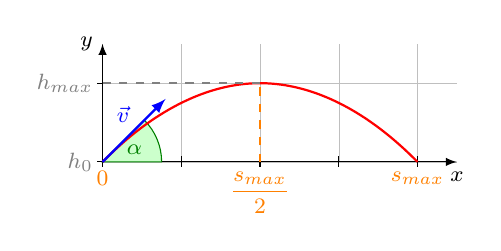
\begin{tikzpicture}
		[
		x=1cm, y=1cm, scale=1.0, font=\footnotesize, >=latex 
		%Voreinstellung für Pfeilspitzen
		]
		
		%Raster im Hintergrund
		\draw[step=1, gray!50!white, very thin] (0,0) grid (4.5,1.5);
		
		
		%Länge x Achse
		\draw [-latex] (0,0) -- ++(4.5,0) node[below] {$x$};
		
		%Länge y Achse
		\draw [-latex] (0,0) -- ++(0,1.5) node[left] {$y$};
		
		%Zahlen auf y-Achse 
		\foreach \y in {0,1}
		\draw[shift={(0,\y)}] (2pt,0pt) -- (-2pt,0pt);
		
		%Zahlen auf x-Achse
		\foreach \x in {0,1,2,3,4}
		\draw[shift={(\x,0)},color=black] (0pt,2pt) -- (0pt,-2pt);
		
		\filldraw[fill=green!20!white, draw=green!50!black] (0,0) -- (0.75,0) arc (0:45:0.75) -- cycle node[midway, below, green!50!black, xshift=4pt, yshift=2pt] {$\alpha$};
		
		%gestrichelte linie
		\draw [dashed, orange, thick] (2,0) -- (2,1);
		
		\draw [] (0,1) node[gray, left] {$h_{max}$};
		\draw [] (0,0) node[gray, left] {$h_{0}$};	
		\draw [] (0,0) node[orange, below] {$0$};
		\draw [] (4,0) node[orange, below] {$s_{max}$};	
		\draw [] (2,0) node[orange, below] {$\dfrac{s_{max}}{2}$};	
		
		% die Parable halt
		\draw[red,thick] (0,0) parabola bend (2,1) (4,0);
		
		\draw [dashed, gray, thick] (2,1)-- (0,1);		
		
		%Vektor v
		\draw[-latex, thick, blue] (0,0) -- (0.8,0.8) node [midway, above, blue, xshift=-4pt, yshift=-1pt] {$\vec{v}$} node (v) {};		
		
\end{tikzpicture}

\end{document}